% Created by tikzDevice version 0.10.1 on 2018-02-07 11:01:34
% !TEX encoding = UTF-8 Unicode
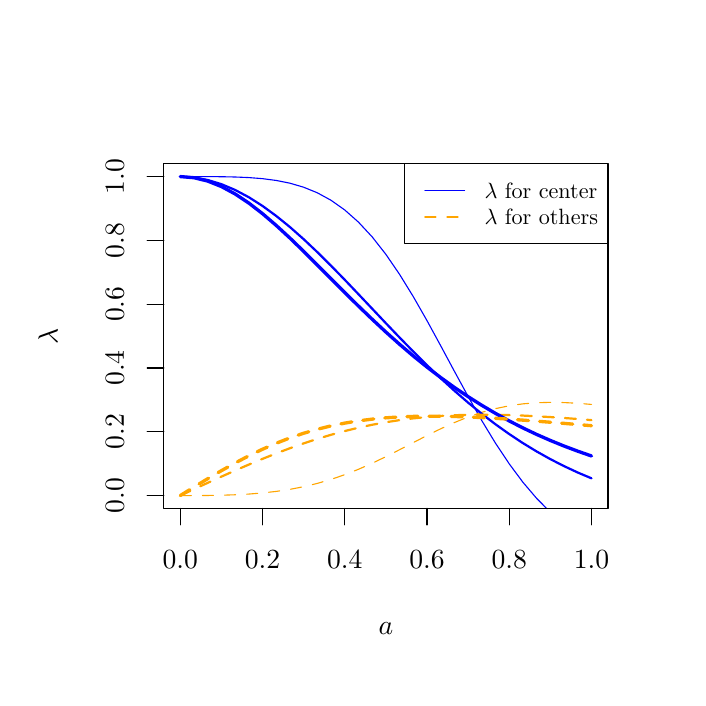
\begin{tikzpicture}[x=1pt,y=1pt]
\definecolor{fillColor}{RGB}{255,255,255}
\path[use as bounding box,fill=fillColor,fill opacity=0.00] (0,0) rectangle (234.88,234.88);
\begin{scope}
\path[clip] ( 49.20, 61.20) rectangle (209.68,185.68);
\definecolor{drawColor}{RGB}{0,0,255}

\path[draw=drawColor,line width= 0.4pt,line join=round,line cap=round] ( 55.14,181.07) --
	( 60.10,181.07) --
	( 65.05,181.06) --
	( 70.00,181.02) --
	( 74.96,180.92) --
	( 79.91,180.71) --
	( 84.86,180.32) --
	( 89.81,179.67) --
	( 94.77,178.68) --
	( 99.72,177.23) --
	(104.67,175.21) --
	(109.63,172.50) --
	(114.58,169.00) --
	(119.53,164.61) --
	(124.49,159.27) --
	(129.44,152.96) --
	(134.39,145.73) --
	(139.34,137.69) --
	(144.30,129.01) --
	(149.25,119.93) --
	(154.20,110.71) --
	(159.16,101.61) --
	(164.11, 92.87) --
	(169.06, 84.70) --
	(174.02, 77.25) --
	(178.97, 70.60) --
	(183.92, 64.78) --
	(188.87, 59.80) --
	(193.83, 55.62) --
	(198.78, 52.15) --
	(203.73, 49.35);
\end{scope}
\begin{scope}
\path[clip] (  0.00,  0.00) rectangle (234.88,234.88);
\definecolor{drawColor}{RGB}{0,0,0}

\path[draw=drawColor,line width= 0.4pt,line join=round,line cap=round] ( 55.14, 61.20) -- (203.73, 61.20);

\path[draw=drawColor,line width= 0.4pt,line join=round,line cap=round] ( 55.14, 61.20) -- ( 55.14, 55.20);

\path[draw=drawColor,line width= 0.4pt,line join=round,line cap=round] ( 84.86, 61.20) -- ( 84.86, 55.20);

\path[draw=drawColor,line width= 0.4pt,line join=round,line cap=round] (114.58, 61.20) -- (114.58, 55.20);

\path[draw=drawColor,line width= 0.4pt,line join=round,line cap=round] (144.30, 61.20) -- (144.30, 55.20);

\path[draw=drawColor,line width= 0.4pt,line join=round,line cap=round] (174.02, 61.20) -- (174.02, 55.20);

\path[draw=drawColor,line width= 0.4pt,line join=round,line cap=round] (203.73, 61.20) -- (203.73, 55.20);

\node[text=drawColor,anchor=base,inner sep=0pt, outer sep=0pt, scale=  1.00] at ( 55.14, 39.60) {0.0};

\node[text=drawColor,anchor=base,inner sep=0pt, outer sep=0pt, scale=  1.00] at ( 84.86, 39.60) {0.2};

\node[text=drawColor,anchor=base,inner sep=0pt, outer sep=0pt, scale=  1.00] at (114.58, 39.60) {0.4};

\node[text=drawColor,anchor=base,inner sep=0pt, outer sep=0pt, scale=  1.00] at (144.30, 39.60) {0.6};

\node[text=drawColor,anchor=base,inner sep=0pt, outer sep=0pt, scale=  1.00] at (174.02, 39.60) {0.8};

\node[text=drawColor,anchor=base,inner sep=0pt, outer sep=0pt, scale=  1.00] at (203.73, 39.60) {1.0};

\path[draw=drawColor,line width= 0.4pt,line join=round,line cap=round] ( 49.20, 65.81) -- ( 49.20,181.07);

\path[draw=drawColor,line width= 0.4pt,line join=round,line cap=round] ( 49.20, 65.81) -- ( 43.20, 65.81);

\path[draw=drawColor,line width= 0.4pt,line join=round,line cap=round] ( 49.20, 88.86) -- ( 43.20, 88.86);

\path[draw=drawColor,line width= 0.4pt,line join=round,line cap=round] ( 49.20,111.91) -- ( 43.20,111.91);

\path[draw=drawColor,line width= 0.4pt,line join=round,line cap=round] ( 49.20,134.96) -- ( 43.20,134.96);

\path[draw=drawColor,line width= 0.4pt,line join=round,line cap=round] ( 49.20,158.02) -- ( 43.20,158.02);

\path[draw=drawColor,line width= 0.4pt,line join=round,line cap=round] ( 49.20,181.07) -- ( 43.20,181.07);

\node[text=drawColor,rotate= 90.00,anchor=base,inner sep=0pt, outer sep=0pt, scale=  1.00] at ( 34.80, 65.81) {0.0};

\node[text=drawColor,rotate= 90.00,anchor=base,inner sep=0pt, outer sep=0pt, scale=  1.00] at ( 34.80, 88.86) {0.2};

\node[text=drawColor,rotate= 90.00,anchor=base,inner sep=0pt, outer sep=0pt, scale=  1.00] at ( 34.80,111.91) {0.4};

\node[text=drawColor,rotate= 90.00,anchor=base,inner sep=0pt, outer sep=0pt, scale=  1.00] at ( 34.80,134.96) {0.6};

\node[text=drawColor,rotate= 90.00,anchor=base,inner sep=0pt, outer sep=0pt, scale=  1.00] at ( 34.80,158.02) {0.8};

\node[text=drawColor,rotate= 90.00,anchor=base,inner sep=0pt, outer sep=0pt, scale=  1.00] at ( 34.80,181.07) {1.0};

\path[draw=drawColor,line width= 0.4pt,line join=round,line cap=round] ( 49.20, 61.20) --
	(209.68, 61.20) --
	(209.68,185.68) --
	( 49.20,185.68) --
	( 49.20, 61.20);
\end{scope}
\begin{scope}
\path[clip] (  0.00,  0.00) rectangle (234.88,234.88);
\definecolor{drawColor}{RGB}{0,0,0}

\node[text=drawColor,anchor=base,inner sep=0pt, outer sep=0pt, scale=  1.00] at (129.44, 15.60) {$a$};

\node[text=drawColor,rotate= 90.00,anchor=base,inner sep=0pt, outer sep=0pt, scale=  1.00] at ( 10.80,123.44) {$\lambda$};
\end{scope}
\begin{scope}
\path[clip] ( 49.20, 61.20) rectangle (209.68,185.68);
\definecolor{drawColor}{RGB}{255,165,0}

\path[draw=drawColor,line width= 0.4pt,dash pattern=on 4pt off 4pt ,line join=round,line cap=round] ( 55.14, 65.81) --
	( 60.10, 65.81) --
	( 65.05, 65.84) --
	( 70.00, 65.93) --
	( 74.96, 66.09) --
	( 79.91, 66.35) --
	( 84.86, 66.75) --
	( 89.81, 67.31) --
	( 94.77, 68.05) --
	( 99.72, 69.01) --
	(104.67, 70.20) --
	(109.63, 71.65) --
	(114.58, 73.35) --
	(119.53, 75.30) --
	(124.49, 77.49) --
	(129.44, 79.87) --
	(134.39, 82.38) --
	(139.34, 84.95) --
	(144.30, 87.50) --
	(149.25, 89.94) --
	(154.20, 92.19) --
	(159.16, 94.19) --
	(164.11, 95.88) --
	(169.06, 97.23) --
	(174.02, 98.25) --
	(178.97, 98.95) --
	(183.92, 99.35) --
	(188.87, 99.49) --
	(193.83, 99.41) --
	(198.78, 99.15) --
	(203.73, 98.74);
\definecolor{drawColor}{RGB}{0,0,255}

\path[draw=drawColor,line width= 0.8pt,line join=round,line cap=round] ( 55.14,181.07) --
	( 60.10,180.76) --
	( 65.05,179.84) --
	( 70.00,178.33) --
	( 74.96,176.24) --
	( 79.91,173.61) --
	( 84.86,170.46) --
	( 89.81,166.85) --
	( 94.77,162.83) --
	( 99.72,158.45) --
	(104.67,153.77) --
	(109.63,148.85) --
	(114.58,143.77) --
	(119.53,138.57) --
	(124.49,133.32) --
	(129.44,128.08) --
	(134.39,122.91) --
	(139.34,117.84) --
	(144.30,112.92) --
	(149.25,108.19) --
	(154.20,103.67) --
	(159.16, 99.38) --
	(164.11, 95.34) --
	(169.06, 91.55) --
	(174.02, 88.02) --
	(178.97, 84.75) --
	(183.92, 81.74) --
	(188.87, 78.97) --
	(193.83, 76.44) --
	(198.78, 74.13) --
	(203.73, 72.04);
\definecolor{drawColor}{RGB}{255,165,0}

\path[draw=drawColor,line width= 0.8pt,dash pattern=on 4pt off 4pt ,line join=round,line cap=round] ( 55.14, 65.81) --
	( 60.10, 68.11) --
	( 65.05, 70.40) --
	( 70.00, 72.65) --
	( 74.96, 74.86) --
	( 79.91, 77.00) --
	( 84.86, 79.07) --
	( 89.81, 81.04) --
	( 94.77, 82.91) --
	( 99.72, 84.66) --
	(104.67, 86.28) --
	(109.63, 87.77) --
	(114.58, 89.12) --
	(119.53, 90.33) --
	(124.49, 91.39) --
	(129.44, 92.30) --
	(134.39, 93.07) --
	(139.34, 93.70) --
	(144.30, 94.20) --
	(149.25, 94.58) --
	(154.20, 94.84) --
	(159.16, 94.98) --
	(164.11, 95.04) --
	(169.06, 95.00) --
	(174.02, 94.89) --
	(178.97, 94.71) --
	(183.92, 94.46) --
	(188.87, 94.17) --
	(193.83, 93.84) --
	(198.78, 93.47) --
	(203.73, 93.07);
\definecolor{drawColor}{RGB}{0,0,255}

\path[draw=drawColor,line width= 1.2pt,line join=round,line cap=round] ( 55.14,181.07) --
	( 60.10,180.66) --
	( 65.05,179.45) --
	( 70.00,177.47) --
	( 74.96,174.79) --
	( 79.91,171.50) --
	( 84.86,167.67) --
	( 89.81,163.42) --
	( 94.77,158.85) --
	( 99.72,154.06) --
	(104.67,149.12) --
	(109.63,144.14) --
	(114.58,139.17) --
	(119.53,134.28) --
	(124.49,129.51) --
	(129.44,124.89) --
	(134.39,120.47) --
	(139.34,116.24) --
	(144.30,112.23) --
	(149.25,108.45) --
	(154.20,104.88) --
	(159.16,101.54) --
	(164.11, 98.41) --
	(169.06, 95.49) --
	(174.02, 92.77) --
	(178.97, 90.24) --
	(183.92, 87.89) --
	(188.87, 85.72) --
	(193.83, 83.70) --
	(198.78, 81.84) --
	(203.73, 80.11);
\definecolor{drawColor}{RGB}{255,165,0}

\path[draw=drawColor,line width= 1.2pt,dash pattern=on 4pt off 4pt ,line join=round,line cap=round] ( 55.14, 65.81) --
	( 60.10, 68.88) --
	( 65.05, 71.89) --
	( 70.00, 74.80) --
	( 74.96, 77.57) --
	( 79.91, 80.17) --
	( 84.86, 82.55) --
	( 89.81, 84.71) --
	( 94.77, 86.64) --
	( 99.72, 88.32) --
	(104.67, 89.77) --
	(109.63, 90.99) --
	(114.58, 91.99) --
	(119.53, 92.80) --
	(124.49, 93.43) --
	(129.44, 93.90) --
	(134.39, 94.22) --
	(139.34, 94.41) --
	(144.30, 94.49) --
	(149.25, 94.48) --
	(154.20, 94.38) --
	(159.16, 94.21) --
	(164.11, 93.99) --
	(169.06, 93.72) --
	(174.02, 93.40) --
	(178.97, 93.06) --
	(183.92, 92.69) --
	(188.87, 92.30) --
	(193.83, 91.89) --
	(198.78, 91.47) --
	(203.73, 91.05);
\definecolor{drawColor}{RGB}{0,0,0}

\path[draw=drawColor,line width= 0.4pt,line join=round,line cap=round] (136.31,185.68) rectangle (209.68,156.88);
\definecolor{drawColor}{RGB}{0,0,255}

\path[draw=drawColor,line width= 0.4pt,line join=round,line cap=round] (143.51,176.08) -- (157.91,176.08);
\definecolor{drawColor}{RGB}{255,165,0}

\path[draw=drawColor,line width= 0.4pt,dash pattern=on 4pt off 4pt ,line join=round,line cap=round] (143.51,166.48) -- (157.91,166.48);
\definecolor{drawColor}{RGB}{0,0,0}

\node[text=drawColor,anchor=base west,inner sep=0pt, outer sep=0pt, scale=  0.80] at (165.11,173.32) {$\lambda$ for center};

\node[text=drawColor,anchor=base west,inner sep=0pt, outer sep=0pt, scale=  0.80] at (165.11,163.72) {$\lambda$ for others};
\end{scope}
\end{tikzpicture}
